\input{style/settings}
\input{style/short_commands}
\pagestyle{fancy}
\fancyhf{}
\fancyhead[R]{página\;\thepage/\pageref{LastPage}}
\fancyhead[L]{Osvaldo Uriel Calderón Dorantes}
\fancyfoot[L]{Seguridad Radiológica}
\fancyfoot[R]{Facultad de Ciencias, UNAM 
\includegraphics[scale=0.13]{style/Sheikah.pdf}}
\fancypagestyle{plain}{
  \fancyfoot[C]{}
}
\makeatletter
\def\@seccntformat#1{%
  \expandafter\ifx\csname c@#1\endcsname\c@section\else
  \csname the#1\endcsname\quad
  \fi}
\makeatother
%%%%%%%%%%%%%%%%%%%%%%%%%%%%%%%%%%%%%%%%%%%%%%%%%%%%%%%
%%%%%%%%%%%%%%%%%%%%%%%%%%%%%%%%%%%%%%%%%%%%%%%%%%%%%%%%%%%
\begin{document}
\begin{flushleft}
Osvaldo Uriel Calderón Dorantes, \hfill Seguridad Radiológica\\
316005171 \hfill osvaldo13576@ciencias.unam  \\
Facultad de Ciencias\\
\underline{Universidad Nacional Autónoma de México}
\end{flushleft}

\begin{flushright}\vspace{-5mm}

\includegraphics[height=1.5cm]{style/logo.pdf}
\end{flushright}
 
\begin{center}\vspace{-1cm}
\textbf{ \large \customfont{Práctica 3\\
Detectores de radiación y levantamiento de niveles}}\\
\today
\end{center}
%\medskip\hrule\medskip
%%%%%%%%%%%%%%%%%%%%%%%%%%%%%%%%%%%%%%%%%%%%%%%%
%{\small \textbf{Nota: A las unidades las pondré dentro de corchetes \ec{[\tx{unidad}]} para no confundir entre variables y realizar el análisis dimensional fácilmente.}}
\medskip\hrule\bigskip

\newlength{\strutheight}
\settoheight{\strutheight}{\strut}
\begin{multicols}{2}

  \section{Introducción}
  \subsection{Exposición \texorpdfstring{\ec{X}}{TEXT}}

  \citep{detec1}


  \subsection{Detector Geiger Muller}

  \subsection{Metodología}

  \section{Resultados}

  \begin{figure}[H]
    \centering
    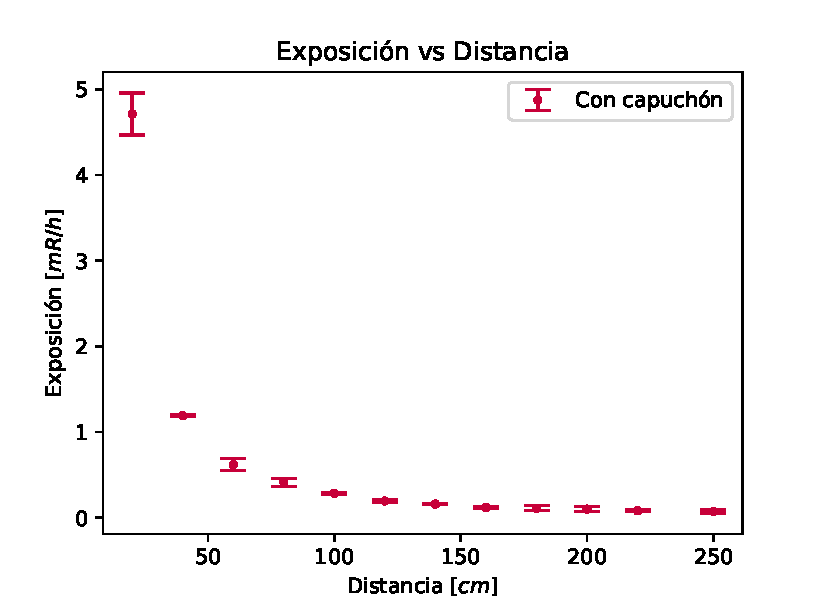
\includegraphics[width=0.45\textwidth]{./figuras/pract_03_con.pdf}
    \caption{Exposición con capuchón en el detector.}
    \label{fig:pract_03_con}
  \end{figure}

  \begin{figure}[H]
    \centering
    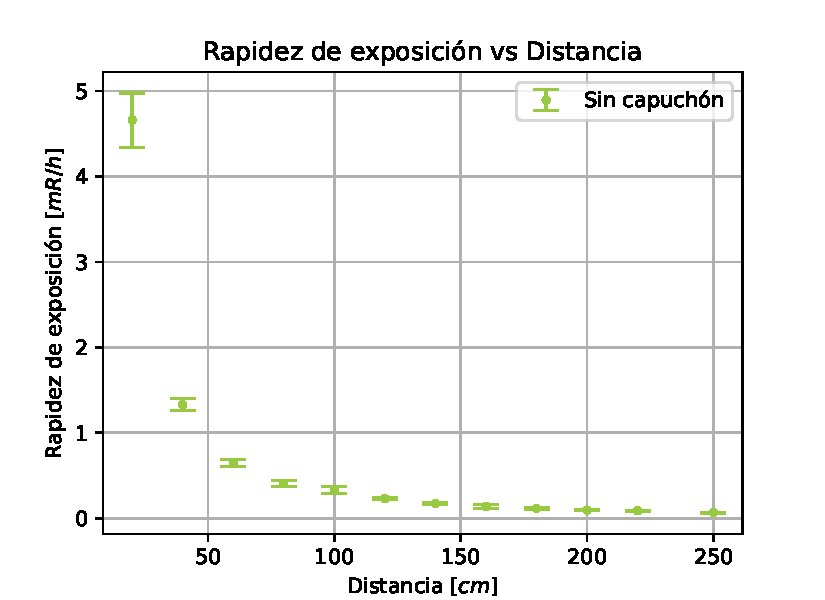
\includegraphics[width=0.45\textwidth]{./figuras/pract_03_sin.pdf}
    \caption{Exposición sin capuchón en el detector.}
    \label{fig:pract_03_sin}
  \end{figure}


  \begin{figure}[H]
    \centering
    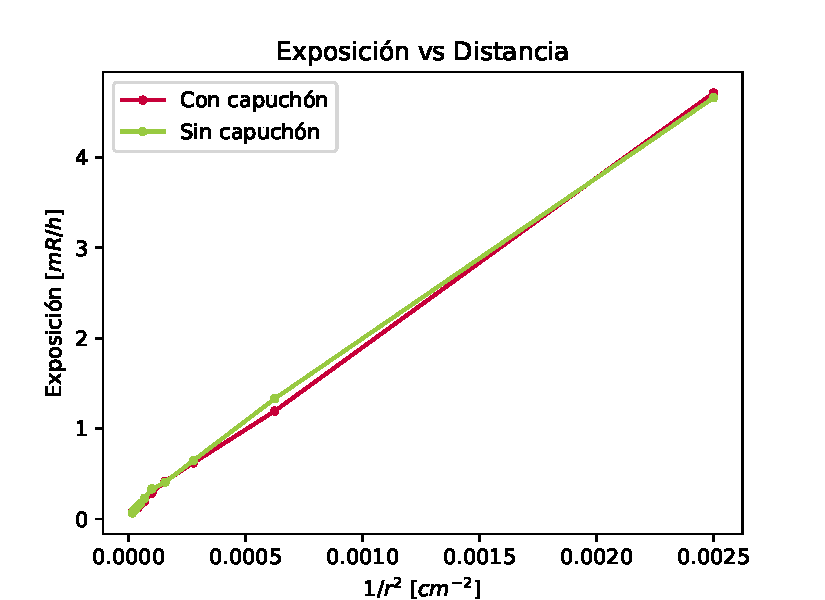
\includegraphics[width=0.45\textwidth]{./figuras/pract_03_code0_rep_r2.pdf}
    \caption{Linealización por cambio de escala del inverso cuadrado de la distancia.}
    \label{fig:pract_r2}
  \end{figure}


  \section{Conclusiones y discusiones} 


\small{\bibliographystyle{apalike}
\bibliography{bib}}
\end{multicols}



%\ftikz{1.5}{figuras/fig.tikz}{}{fig:x}

\end{document}



